\documentclass[12pt,a4paper]{article}
\usepackage[english]{babel}
\usepackage[T1]{fontenc}
\usepackage[utf8]{inputenc}
\usepackage[htt]{hyphenat}

\pagestyle{headings}

\usepackage{graphicx} % Required for including pictures
\graphicspath{{Pictures/}} % Specifies the directory where pictures are stored

\usepackage{listings}

\usepackage[hidelinks, pdfencoding=unicode]{hyperref}
\usepackage[bottom]{footmisc}

\usepackage{tikz}
\usetikzlibrary{positioning}

\newcommand*\justify{%
  \fontdimen2\font=0.4em% interword space
  \fontdimen3\font=0.2em% interword stretch
  \fontdimen4\font=0.1em% interword shrink
  \fontdimen7\font=0.1em% extra space
  \hyphenchar\font=`\-% allowing hyphenation
}

\makeatletter 
\newcommand\mynobreakpar{\par\nobreak\@afterheading} 
\makeatother

\usepackage{gensymb}

\begin{document}

%----------------------------------------------------------------------------------------
%	TITLE PAGE
%----------------------------------------------------------------------------------------

\begin{titlepage}

\newcommand{\HRule}{\rule{\linewidth}{0.5mm}} % Defines a new command for the horizontal lines, change thickness here

\center % Center everything on the page


\includegraphics[width=0.5\textwidth]{mdh_logo}~\\[2cm] % Include a department/university logo - this will require the graphicx package

\textsc{\Large DVA427 --- Assignment 5}\\[0cm]


\HRule \\[0.8cm]
\begin{center}
 \Huge \bfseries Reinforcement Learning\par Inverted Pendulum\\[0.4cm] % Title of your document
\end{center}
\HRule \\[0.5cm]

\vspace{\fill}

\begin{minipage}{0.4\textwidth}
\begin{flushleft} \large
\emph{Authors:}\\
Petr \textsc{Fejfar}\\[0.2cm] % Your name
Martin \textsc{Váňa}\\[0.2cm] % Your name
\end{flushleft}
\end{minipage}
~
\begin{minipage}{0.4\textwidth}
\begin{flushright} \large
~\\
~\\
\emph{Datum:} \\
\today\\[0.2cm] % Date, change the \today to a set date if you want to be precise
\end{flushright}
\end{minipage}\\

\end{titlepage}


%----------------------------------------------------------------------------------------
%	TOC
%----------------------------------------------------------------------------------------
\thispagestyle{empty}

\tableofcontents


\newpage


\setcounter{page}{3}

%----------------------------------------------------------------------------------------
%	TASK
%----------------------------------------------------------------------------------------

\section{Task}

In this assignment you will apply the reinforcement learning technique to learn optimal
action strategies for automatic control. The plant to be considered is an inverted pendulum
system. The constitution of the pendulum system is depicted in the following figure, where a
pole is hinged to a cart which moves on a rail to its right and left. The pole has only one
degree of freedom to rotate around the hinge point. The controller can apply a ''left'' or
''right'' force of fixed magnitude to the cart at discrete time intervals. 

\begin{figure}[!ht]
\centering
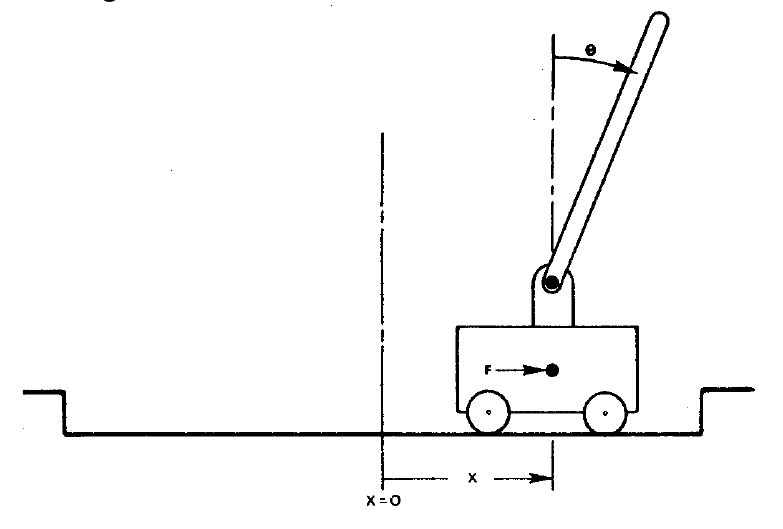
\includegraphics[width=.6\textwidth]{pendulum-system.jpg}
\caption{The constitution of the pendulum system}
\label{img:pendulum_system}
\end{figure}

\noindent
The states of the pendulum system are:
\begin{enumerate}

	\item position of the cart($x$)
	\item angle of the pole ($\theta$)
	\item cart velocity on the rail ($\dot x$)
	\item speed of pole rotation ($\dot \theta$)

\end{enumerate}

\noindent
We can use such states to describe the behaviour of the system as a set of non-linear
differential equations as

$$
\ddot{\theta}(t) = \frac{ g\,sin(\theta(t)) + cos(\theta(t))\Big[\frac{-F(t)-ml\dot{\theta}(t)^2sin(\theta(t))}{m_c + m}\Big]}
                        {l\Big[\frac{4}{3} - \frac{m\,cos(\theta(t))^2}{m_c + m}\Big]}
$$

$$
\ddot{x}(t) = \frac{F(t) + ml \lfloor \dot\theta(t)^2 sin(\theta(t)) - \ddot{\theta}(t) cos(\theta(t))\rfloor}
                   {m_c + m}
$$

\noindent
Where\mynobreakpar
\begin{itemize}

	\item[] $g = -9.8 \frac{m}{s^2}$, acceleration due to gravity
	\item[] $m_c = 10 kg$, mass of the cart
	\item[] $m = 0.1 kg$, mass of the pole
	\item[] $l = 0.5 m$ , half of the pole length
	\item[] $F(t) = +10 N$ or $-10 N$, force applied to cart’s mass center at time t.

\end{itemize}

The system survives if the cart position is within $[-2.4 m, 2.4 m]$ and pole angle is not more
than $12$ degrees. Suppose the initiate state of the system is $(x=0,\, \dot x=0,\, \theta=0,\, \dot \theta=0)$ and the 
discrete time interval is $0.02$ second. Now your task is to use the reinforcement learning
method to learn the best strategy of selecting forces such that the survival time of the system
is maximized.


In order to get response of the system by applying a force under a state, you have to do
simulation of the real plant in terms of the system equations given above. A simulation
function in MATLAB code is available from the ''Labs'' folder. But you have to program the
simulation function if you use other languages in this assignment.


Your report has to clarify your approach and results by covering the following issues:

\begin{enumerate}

	\item How do you characterize (discretize) states of the world in this learning task?
	\item What is the reward function designed?
	\item What is the function to be learned?
	\item What learning algorithm is used?
	\item How do you choose exploratory actions?
	\item How many intervals can your system survive by using the learned strategy?

\end{enumerate}
%----------------------------------------------------------------------------------------
%	ANALYSIS
%----------------------------------------------------------------------------------------

\newpage

\section{Analysis}

\subsection{State discretization}

We have constricted continuous variables with reasonable values and then divided uniformly.

\begin{enumerate}

	\item position of the cart($x$) --- constraints $\langle-2.4, 2.4\rangle$, $8$ intervals
	\item angle of the pole ($\theta$) --- constraints $\langle-12\degree, 12\degree\rangle$, $28$ intervals
	\item cart velocity on the rail ($\dot x$) --- constraints $\langle-1, 1\rangle$, $10$ intervals
	\item speed of pole rotation ($\dot \theta$) --- constraints $\langle-1, 1\rangle$, $28$ intervals

\end{enumerate}


\subsection{Reward function}

Our reward function is simple. It returns $1$ if the state is safe, $0$ otherwise.


\subsection{Q function}

$Q^*(s,a)$ is the expected pay-off when taking the action $a$ at the state $s$ and following the optimal policy $\pi^*$.

$$
Q(s,a) = Q(s,a) + \alpha[r^a_{ss'} + \gamma \max_{a}Q^*(s',a') - Q(s,a)]
$$

\noindent
,where $s, s'$ are states, $a,a'$ are actions, $\alpha$ is learning rate and $\gamma$ is a discount factor and $r^a_{ss'}$ is a reward.

\subsection{Learning algorithm}

As learning algorithm we are using stochastic Q-learning. Due to state discretization state transition is not deterministic. Although system state transition function is deterministic, transition from discrete system state can end in multiple states. 


We run 6000 simulation and we stop simulation when it reach $30000^{th}$ state. These parameters are set to target achieve 2 minutes long run, which is consireded to stable run.

$\gamma$ we set to $0.1$. State $a_0$ is move with cart by force $-10N$ and $a_1$ is move with cart by force $10N$.

\subsection{Random action selection}

For exploring new states we are using \href{distriburion https://en.wikipedia.org/wiki/Boltzmann\_distribution}{Boltzmann distribution}

$$
p_i = \frac{e^{-\epsilon_i/kT}}
                        {\sum\limits_{i=0}^N e^{-\epsilon_i/kT}}
$$

\noindent
,where $p_i$ is probability that action $a_i$ is chosen. $\epsilon_i$ is energy of state which we set to actual $Q(s, a_i)$, $k$ is Boltzmann constant and $T$ is temperature of system which we set empirically. Boltzmann constant $k$ is not relevant to our problem so we set is to $1$.

\subsection{Visualization}

Debugging of the algorithm is very challenging process, so we created visualization (Figure 2). State $s$ has 4 dimension, but resolution isn't high. We chose to show 2 dimension per axis. We split graph by grid which represent states of the first dimension. Inside each grid splitted cell we show whole second dimension for current state in first dimension (Figure 3). Same process we did for second axis. Color represents difference $Q(s, a_0) - Q(s, a_1)$.

\begin{figure}[!ht]
\centering
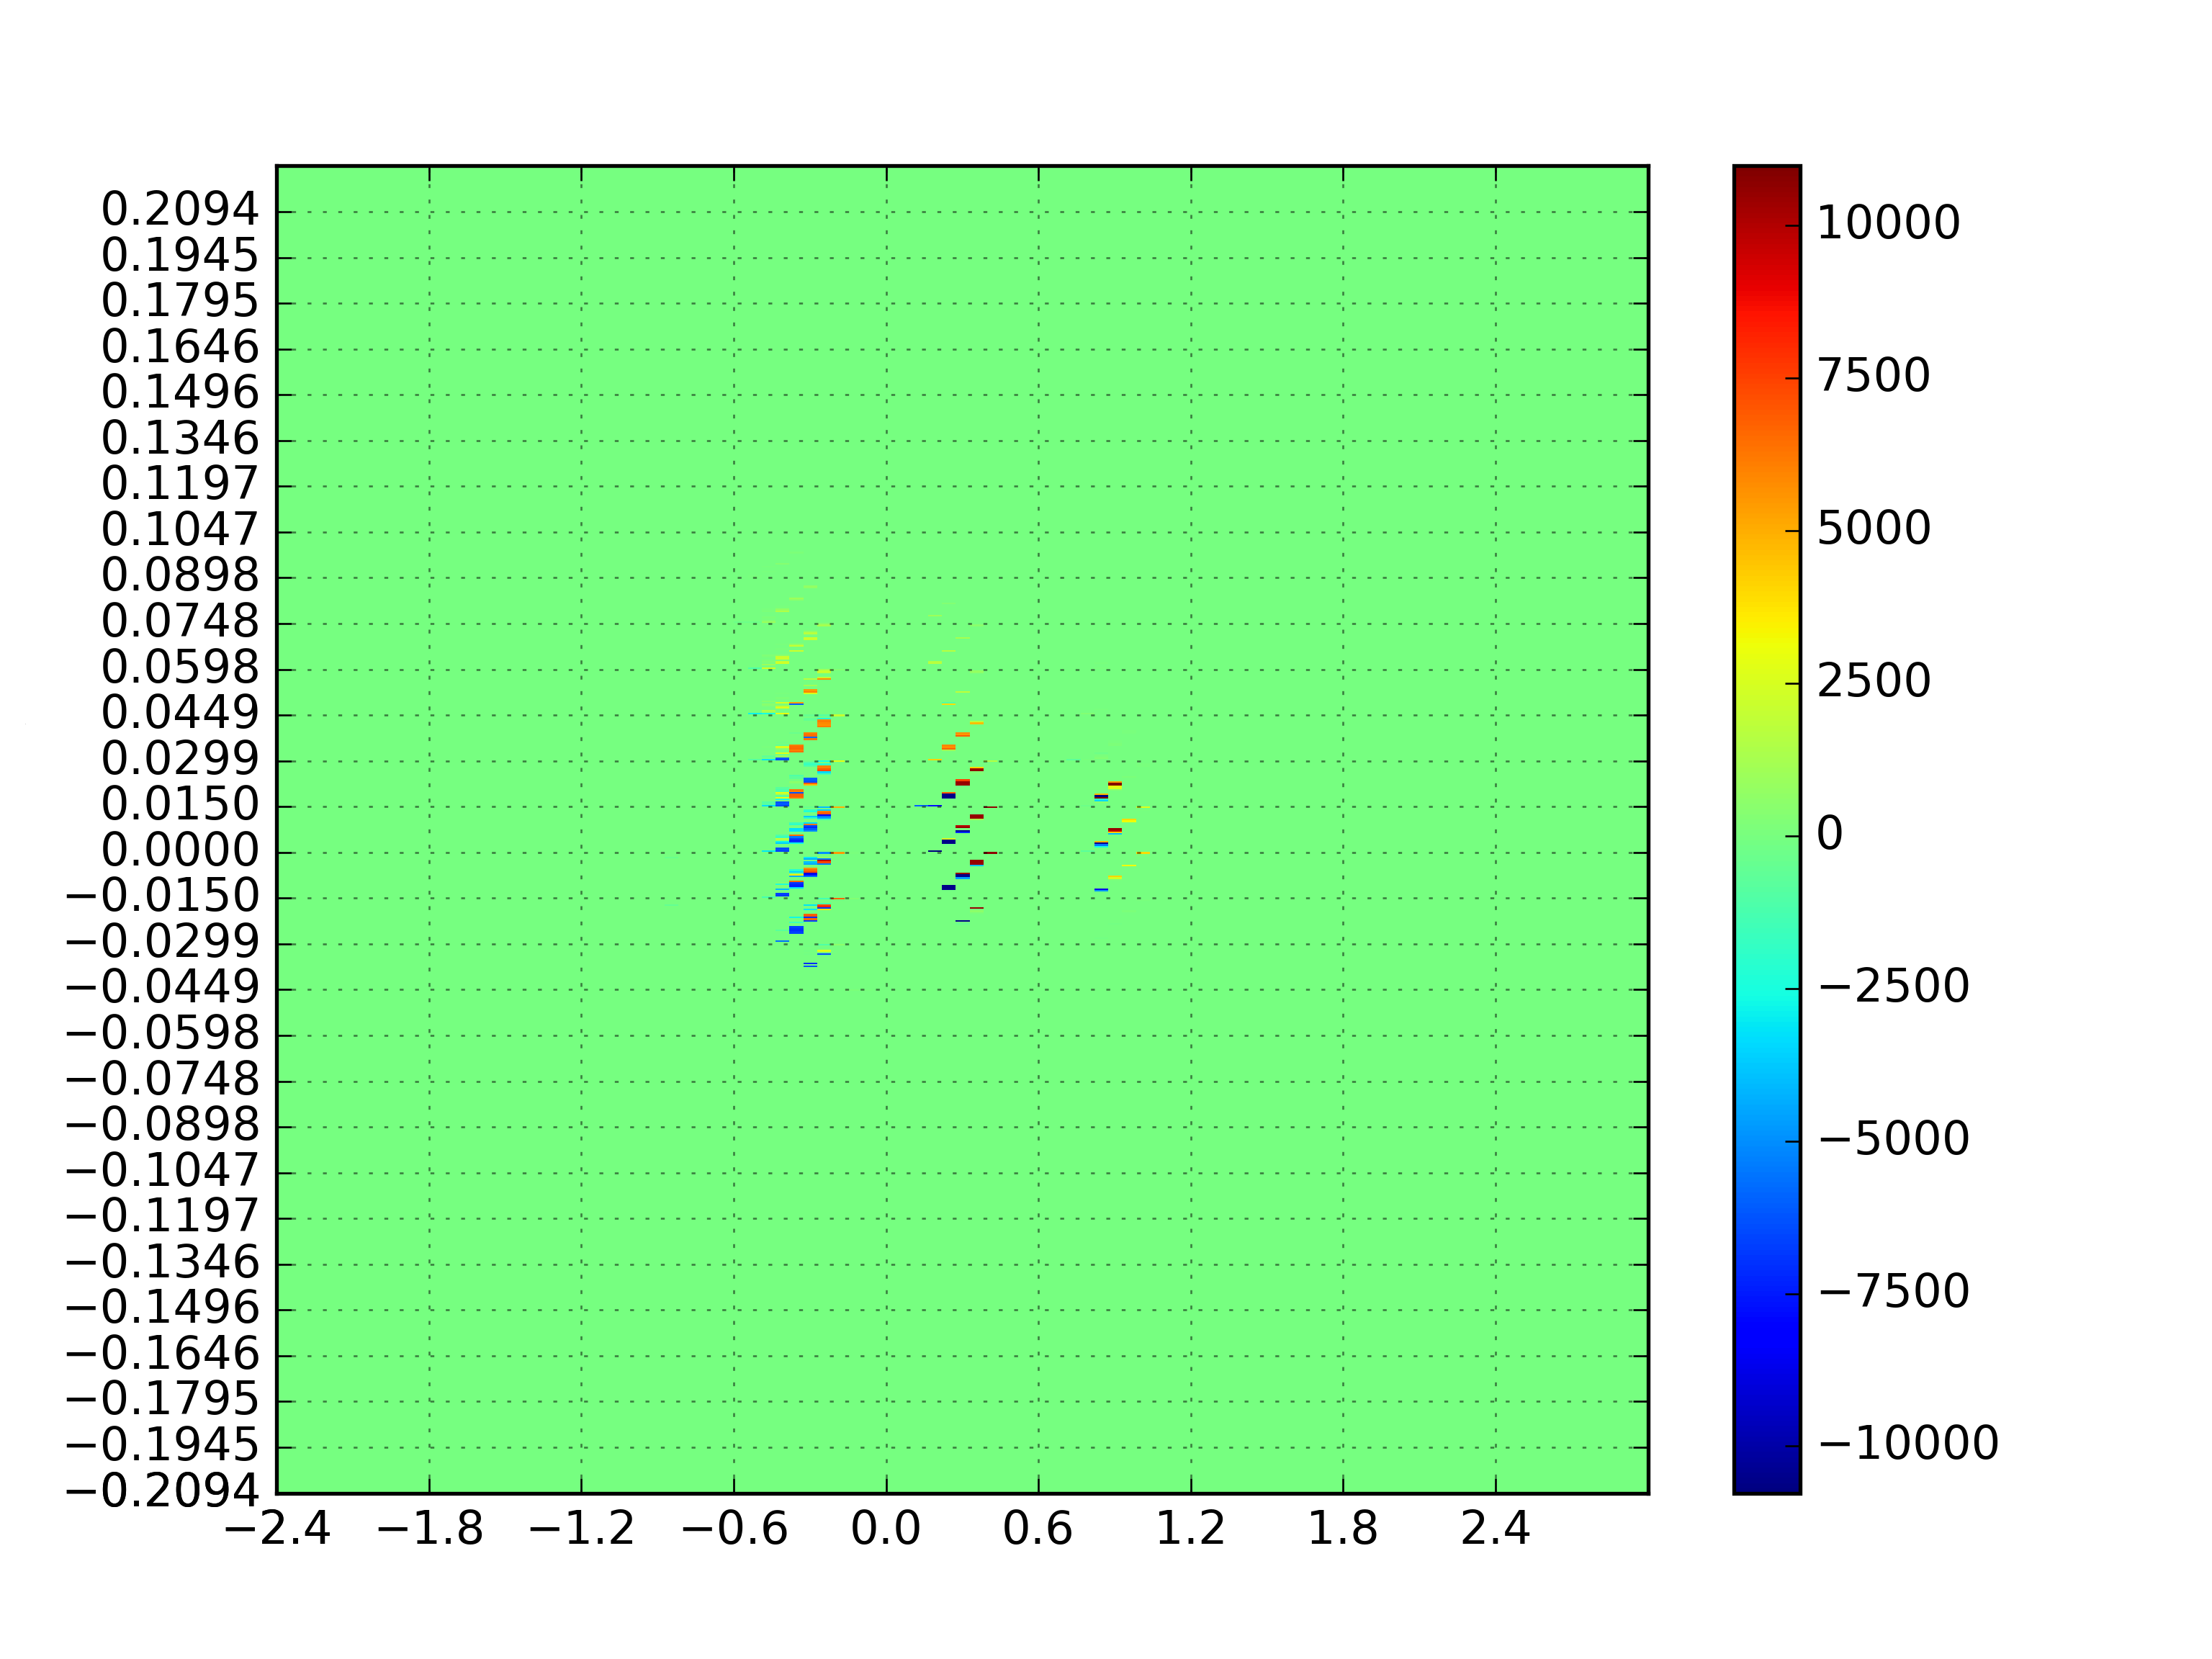
\includegraphics[width=1.0\textwidth]{visualization.png}
\caption{Visualization of state of $Q(s, a)$, where $x$ axis is position/speed and $y$ axis is angle/angle speed.}
\label{img:visualization}
\end{figure}

\begin{figure}[!ht]
\centering
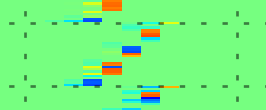
\includegraphics[width=0.2\textwidth]{visualization-zoom.png}
\caption{Detail of cell in visualization of state of $Q(s, a)$, where $x$ axis is speed and $y$ axis is angle speed.}
\label{img:visualization}
\end{figure}

\subsection{Results}

Algorithm can achieve 2 minutes run. After 2 minutes we stop the simulation. We attach video with 2 minutes run achieved by our algorithm to this document.

%----------------------------------------------------------------------------------------
%	CONCLUSION
%----------------------------------------------------------------------------------------

\section{Conclusion}

From visualization we learned that Q-learning algorithm fill more states near state $(0, 0, 0, 0)$. This is resulting in pendulum crash after leaving neighbourhood of state $(0, 0, 0, 0)$. Algorithm was very stable on states where was trained properly. 


\section{Future work}

We want to face problem of not learning all states. We suggest to use backtracking of all possible state during state exploration phase. This is possible because of we don't use physical system, but simulated one. Next thing we want to focus is to make pendulum stay near state $(0, 0, 0, 0)$, where is trained. We want to achieve that by rewarding system to stay close to $(0, 0, 0, 0)$


% autorův rozbor dosažených výsledků, vyzdvihnutí kladů a přínosu prezentovaného řešení,  kritika nedostatků ap.

% zhodnocení, jak bylo splněno zadání
% možnosti dalšího rozvoje prezentovaného řešení ap.

\end{document}
